%%%%%%%%%%%%%%%%%%%%%%%%%%%%%%%%%%%%%%%%%%%%%%%%%%%%%%%%%%%%%%%%%%%%%%%%
% Plantilla TFG/TFM
% Universidad de Murcia. Facultad de Informática
% Realizado por: José Manuel Requena Plens
% Modificado: Pablo José Rocamora Zamora
% Contacto: pablojoserocamora@gmail.com
%%%%%%%%%%%%%%%%%%%%%%%%%%%%%%%%%%%%%%%%%%%%%%%%%%%%%%%%%%%%%%%%%%%%%%%%

\chapter{Análisis de objetivos y metodología}
\label{cap:analisis}

Este capítulo detalla el análisis previo a la implementación del sistema, describiendo la metodología de trabajo adoptada y los requisitos funcionales y no funcionales que han guiado el desarrollo del chatbot basado en Grafos de Conocimiento.

\section{Metodología de Desarrollo}

Dada la naturaleza exploratoria de este Trabajo de Fin de Grado, centrado en la integración de Inteligencia Artificial Generativa y Web Semántica, la adopción de una metodología clásica en cascada (\textit{Waterfall}) resultaba inapropiada. El comportamiento de los Modelos de Lenguaje de Gran Escala (LLMs) es no determinista y requiere de experimentación continua, especialmente en el ámbito de la ingeniería de \textit{prompts} y la extracción de datos.

Por ello, se ha optado por un \textbf{enfoque ágil e iterativo basado en prototipos}. El desarrollo se ha dividido en ciclos cortos de experimentación:
\begin{enumerate}
    \item \textbf{Exploración y Extracción de Datos:} Pruebas iniciales para consultar Wikidata y consolidar un Grafo de Conocimiento local funcional y acotado.
    \item \textbf{Prototipado del Agente:} Desarrollo iterativo del \textit{prompt} principal del LLM para traducir lenguaje natural a SPARQL.
    \item \textbf{Implementación del Bucle de Reflexión:} Adición del mecanismo de autocorrección ante errores de sintaxis en el código generado.
    \item \textbf{Evaluación y Refinamiento:} Pruebas de rendimiento frente al \textit{dataset} de evaluación que derivaron en ajustes continuos en el flujo de ejecución.
\end{enumerate}

Este enfoque ha permitido pivotar rápidamente cuando ciertas estrategias de \textit{prompting} no lograban la precisión requerida en la generación de SPARQL.

\section{Análisis de Requisitos}

Para asegurar que el sistema cumple con los objetivos planteados, se han especificado una serie de requisitos funcionales y no funcionales.

\subsection{Requisitos Funcionales}

Los requisitos funcionales (RF) describen las interacciones y el comportamiento esperado del sistema:

\begin{itemize}
    \item \textbf{RF-01. Interfaz conversacional:} El sistema debe proporcionar una interfaz gráfica que permita al usuario realizar preguntas en lenguaje natural de forma intuitiva, similar a un chat convencional.
    \item \textbf{RF-02. Extracción y desambiguación de entidades:} El sistema debe ser capaz de identificar la entidad principal en la consulta del usuario (ej. nombre de un actor o película) y desambiguarla contra Wikidata para obtener su identificador único (ej. \texttt{wd:Q25191}).
    \item \textbf{RF-03. Generación de SPARQL:} El agente LLM debe traducir la pregunta del usuario en una consulta SPARQL sintáctica y semánticamente válida, usando únicamente las propiedades definidas en el diccionario del sistema.
    \item \textbf{RF-04. Bucle de autocorrección:} Si la consulta SPARQL generada produce un error al ejecutarse en el motor RDF, el agente debe leer el mensaje de error y regenerar la consulta corregida de forma autónoma, sin intervención del usuario.
    \item \textbf{RF-05. Ejecución y respuesta local:} El sistema debe ejecutar las consultas sobre el Grafo de Conocimiento local (\texttt{datos\_cine\_seguro.ttl}) y presentar la respuesta extraída al usuario en un formato legible.
\end{itemize}

\subsection{Requisitos No Funcionales}

Los requisitos no funcionales (RNF) definen las restricciones y atributos de calidad del sistema:

\begin{itemize}
    \item \textbf{RNF-01. Precisión y mitigación de alucinaciones:} El sistema debe priorizar la exactitud del código SPARQL generado, limitando estrictamente el alcance de conocimiento del LLM al esquema de la base de datos local para evitar alucinaciones.
    \item \textbf{RNF-02. Tiempos de respuesta:} El sistema debe mantener tiempos de respuesta aceptables (generalmente inferiores a los 10 segundos), teniendo en cuenta el tiempo requerido para las llamadas a la API del LLM y la desambiguación.
    \item \textbf{RNF-03. Modularidad:} El código debe estar desacoplado, separando la lógica de la interfaz (\texttt{interfaz.py}), la lógica del agente (\texttt{chatLocal.py}) y la extracción de datos (\texttt{entidades\_cine.py}).
\end{itemize}

\section{Casos de Uso}

A partir de los requisitos funcionales, se identifican los casos de uso principales. El caso de uso central del sistema es la \textit{Consulta de información cinematográfica}.



\begin{figure}[h]
    \centering
    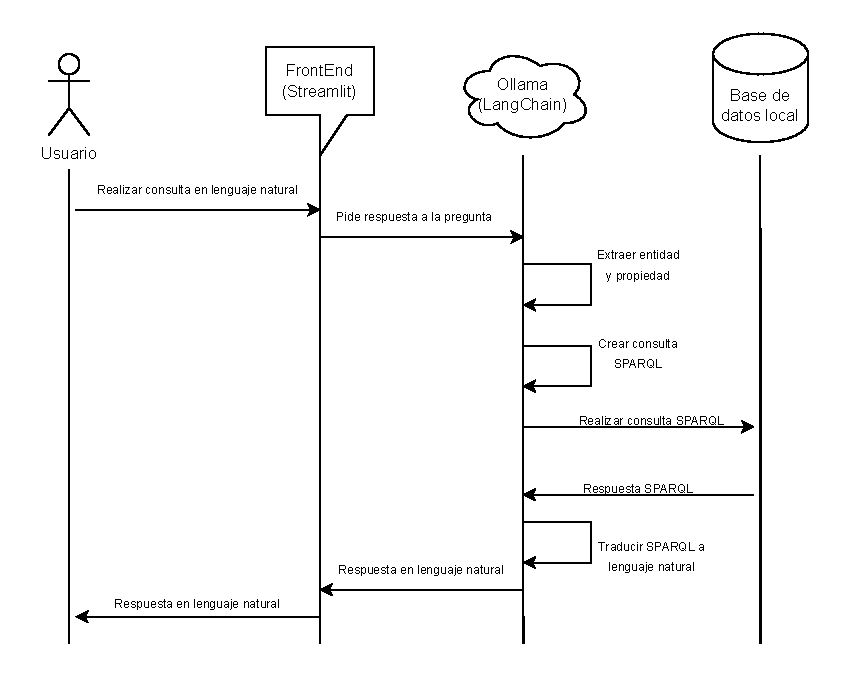
\includegraphics[width=0.9\textwidth]{archivos/CasoDeUso.pdf}
    \caption{Diagrama de Casos de Uso}
    \label{fig:casos_uso}
\end{figure}

En este caso de uso central, el Actor (Usuario) interactúa con la interfaz de chat. El sistema, de forma transparente para el usuario, ejecuta sub-casos como la extracción de entidades, la generación de código y la consulta iterativa al grafo local.